{\textbf{1. 双亲表示法}}{}

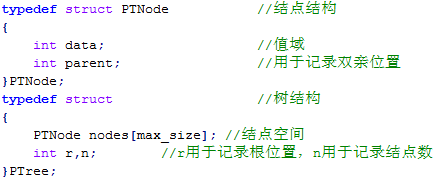
\includegraphics[width=3.70833in,height=1.52083in]{png-jpeg-pics/4836DA8387A9B72CC5286F7A0ADCE5C4.png}

{下图为一棵树及双亲表示法的存储结构。\\
}

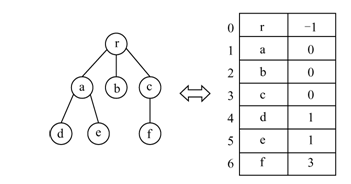
\includegraphics[width=3.65625in,height=1.91667in]{png-jpeg-pics/07F6C48018B2828EBF2C3AE203EC4184.png}

{\textbf{2. 孩子表示法}}

{1)假设d为树的度,采用d叉链表的存储结构,但由于很多结点的度小于d,造成很大的浪费。}

{2)把每个结点的孩子结点排列起来,看成一个线性表,且以单链表做存储结构,则n个结点有n个孩子链表。如下图所示的例子。}

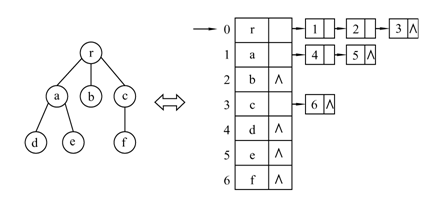
\includegraphics[width=3.70833in,height=1.75000in]{png-jpeg-pics/899A3EB24E8B87B9EC2551F99D4AF3C4.png}

{\textbf{3. 孩子兄弟表示法}}

{~ ~ ~
孩子兄弟表示法又称二叉链表表示法,其实就是把树转换为二叉树,进行存储,如下图所示。}

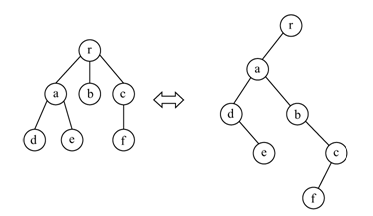
\includegraphics[width=3.70833in,height=2.14583in]{png-jpeg-pics/5658702D90DC100F532749204A4F84F3.png}
